\documentclass[]{elsarticle} %review=doublespace preprint=single 5p=2 column
%%% Begin My package additions %%%%%%%%%%%%%%%%%%%
\usepackage[hyphens]{url}



\usepackage{lineno} % add

\usepackage{graphicx}
%%%%%%%%%%%%%%%% end my additions to header

\usepackage[T1]{fontenc}
\usepackage{lmodern}
\usepackage{amssymb,amsmath}
\usepackage{ifxetex,ifluatex}
\usepackage{fixltx2e} % provides \textsubscript
% use upquote if available, for straight quotes in verbatim environments
\IfFileExists{upquote.sty}{\usepackage{upquote}}{}
\ifnum 0\ifxetex 1\fi\ifluatex 1\fi=0 % if pdftex
  \usepackage[utf8]{inputenc}
\else % if luatex or xelatex
  \usepackage{fontspec}
  \ifxetex
    \usepackage{xltxtra,xunicode}
  \fi
  \defaultfontfeatures{Mapping=tex-text,Scale=MatchLowercase}
  \newcommand{\euro}{€}
\fi
% use microtype if available
\IfFileExists{microtype.sty}{\usepackage{microtype}}{}
\bibliographystyle{elsarticle-harv}
\ifxetex
  \usepackage[setpagesize=false, % page size defined by xetex
              unicode=false, % unicode breaks when used with xetex
              xetex]{hyperref}
\else
  \usepackage[unicode=true]{hyperref}
\fi
\hypersetup{breaklinks=true,
            bookmarks=true,
            pdfauthor={Willem Vervoort/Eliana Nervi/Jimena Alonso},
            pdftitle={Replies to editor and associate editor Journal of Hydrology},
            colorlinks=false,
            urlcolor=blue,
            linkcolor=magenta,
            pdfborder={0 0 0}}
\urlstyle{same}  % don't use monospace font for urls

\setcounter{secnumdepth}{5}
% Pandoc toggle for numbering sections (defaults to be off)

% Pandoc syntax highlighting
\usepackage{color}
\usepackage{fancyvrb}
\newcommand{\VerbBar}{|}
\newcommand{\VERB}{\Verb[commandchars=\\\{\}]}
\DefineVerbatimEnvironment{Highlighting}{Verbatim}{commandchars=\\\{\}}
% Add ',fontsize=\small' for more characters per line
\usepackage{framed}
\definecolor{shadecolor}{RGB}{248,248,248}
\newenvironment{Shaded}{\begin{snugshade}}{\end{snugshade}}
\newcommand{\AlertTok}[1]{\textcolor[rgb]{0.94,0.16,0.16}{#1}}
\newcommand{\AnnotationTok}[1]{\textcolor[rgb]{0.56,0.35,0.01}{\textbf{\textit{#1}}}}
\newcommand{\AttributeTok}[1]{\textcolor[rgb]{0.77,0.63,0.00}{#1}}
\newcommand{\BaseNTok}[1]{\textcolor[rgb]{0.00,0.00,0.81}{#1}}
\newcommand{\BuiltInTok}[1]{#1}
\newcommand{\CharTok}[1]{\textcolor[rgb]{0.31,0.60,0.02}{#1}}
\newcommand{\CommentTok}[1]{\textcolor[rgb]{0.56,0.35,0.01}{\textit{#1}}}
\newcommand{\CommentVarTok}[1]{\textcolor[rgb]{0.56,0.35,0.01}{\textbf{\textit{#1}}}}
\newcommand{\ConstantTok}[1]{\textcolor[rgb]{0.00,0.00,0.00}{#1}}
\newcommand{\ControlFlowTok}[1]{\textcolor[rgb]{0.13,0.29,0.53}{\textbf{#1}}}
\newcommand{\DataTypeTok}[1]{\textcolor[rgb]{0.13,0.29,0.53}{#1}}
\newcommand{\DecValTok}[1]{\textcolor[rgb]{0.00,0.00,0.81}{#1}}
\newcommand{\DocumentationTok}[1]{\textcolor[rgb]{0.56,0.35,0.01}{\textbf{\textit{#1}}}}
\newcommand{\ErrorTok}[1]{\textcolor[rgb]{0.64,0.00,0.00}{\textbf{#1}}}
\newcommand{\ExtensionTok}[1]{#1}
\newcommand{\FloatTok}[1]{\textcolor[rgb]{0.00,0.00,0.81}{#1}}
\newcommand{\FunctionTok}[1]{\textcolor[rgb]{0.00,0.00,0.00}{#1}}
\newcommand{\ImportTok}[1]{#1}
\newcommand{\InformationTok}[1]{\textcolor[rgb]{0.56,0.35,0.01}{\textbf{\textit{#1}}}}
\newcommand{\KeywordTok}[1]{\textcolor[rgb]{0.13,0.29,0.53}{\textbf{#1}}}
\newcommand{\NormalTok}[1]{#1}
\newcommand{\OperatorTok}[1]{\textcolor[rgb]{0.81,0.36,0.00}{\textbf{#1}}}
\newcommand{\OtherTok}[1]{\textcolor[rgb]{0.56,0.35,0.01}{#1}}
\newcommand{\PreprocessorTok}[1]{\textcolor[rgb]{0.56,0.35,0.01}{\textit{#1}}}
\newcommand{\RegionMarkerTok}[1]{#1}
\newcommand{\SpecialCharTok}[1]{\textcolor[rgb]{0.00,0.00,0.00}{#1}}
\newcommand{\SpecialStringTok}[1]{\textcolor[rgb]{0.31,0.60,0.02}{#1}}
\newcommand{\StringTok}[1]{\textcolor[rgb]{0.31,0.60,0.02}{#1}}
\newcommand{\VariableTok}[1]{\textcolor[rgb]{0.00,0.00,0.00}{#1}}
\newcommand{\VerbatimStringTok}[1]{\textcolor[rgb]{0.31,0.60,0.02}{#1}}
\newcommand{\WarningTok}[1]{\textcolor[rgb]{0.56,0.35,0.01}{\textbf{\textit{#1}}}}

% tightlist command for lists without linebreak
\providecommand{\tightlist}{%
  \setlength{\itemsep}{0pt}\setlength{\parskip}{0pt}}

% From pandoc table feature
\usepackage{longtable,booktabs,array}
\usepackage{calc} % for calculating minipage widths
% Correct order of tables after \paragraph or \subparagraph
\usepackage{etoolbox}
\makeatletter
\patchcmd\longtable{\par}{\if@noskipsec\mbox{}\fi\par}{}{}
\makeatother
% Allow footnotes in longtable head/foot
\IfFileExists{footnotehyper.sty}{\usepackage{footnotehyper}}{\usepackage{footnote}}
\makesavenoteenv{longtable}

% Pandoc citation processing
\newlength{\cslhangindent}
\setlength{\cslhangindent}{1.5em}
\newlength{\csllabelwidth}
\setlength{\csllabelwidth}{3em}
\newlength{\cslentryspacingunit} % times entry-spacing
\setlength{\cslentryspacingunit}{\parskip}
% for Pandoc 2.8 to 2.10.1
\newenvironment{cslreferences}%
  {}%
  {\par}
% For Pandoc 2.11+
\newenvironment{CSLReferences}[2] % #1 hanging-ident, #2 entry spacing
 {% don't indent paragraphs
  \setlength{\parindent}{0pt}
  % turn on hanging indent if param 1 is 1
  \ifodd #1
  \let\oldpar\par
  \def\par{\hangindent=\cslhangindent\oldpar}
  \fi
  % set entry spacing
  \setlength{\parskip}{#2\cslentryspacingunit}
 }%
 {}
\usepackage{calc}
\newcommand{\CSLBlock}[1]{#1\hfill\break}
\newcommand{\CSLLeftMargin}[1]{\parbox[t]{\csllabelwidth}{#1}}
\newcommand{\CSLRightInline}[1]{\parbox[t]{\linewidth - \csllabelwidth}{#1}\break}
\newcommand{\CSLIndent}[1]{\hspace{\cslhangindent}#1}




\begin{document}


\begin{frontmatter}

  \title{Replies to editor and associate editor Journal of Hydrology}
    \author[]{}
  
      
  \begin{abstract}
  
  \end{abstract}
  
 \end{frontmatter}

\hypertarget{introduction}{%
\section{Introduction}\label{introduction}}

This document records the replies to the reviewer for the first submission of \emph{``Factors determining how catchments respond to forest cover change. Re-analysing global data sets''} to Journal of Hydrology, which was rejected before review.\\
\strut \\
Reviewer comments in \textcolor{blue}{blue}. Our responses in normal text.\\
\strut \\
\textbf{The most important point from the reviews is the fact that we have not communicated the need for this paper. We need to rewrite the introduction to do this better.}\\
\strut \\

\hypertarget{editor-comments}{%
\section{Editor comments}\label{editor-comments}}

\textcolor{blue}{The first is to streamline the statistics.  As suggested by the AE, a formal model selection process, followed by using only the selected model(s) to evaluate change, would be a suitable approach.}\\
\strut \\
\textbf{check this}
We politely disagree with the suggestion of a formal model selection process, as we outline in our reply to the AE. If the statistical modelling aimed at developing the best predictive model, then this would be the right approach. However, in this case the statistical modelling is aimed at hypothesis testing and explanation of variance in the data set.\\
\strut \\
\textcolor{blue}{In doing so, please carefully note the AEs' concerns about some of the statistical methodology - concerns which range from interpretation to the use of appropriate performance metrics across models of varying structure, to the selection of the appropriate metrics of forest cover change for analysis.}\\
\strut \\
Please see our comments in reply to the AE below.\\
\hspace*{0.333em}
\textcolor{blue}{The second - hopefully supported by a streamlining of the statistics - is to simplify and improve the coherence of the argument.  Framing - as the AE states - a "systematic" exploration of the importance of parameters, will improve the readability and interpretability of the work.  At present, I think because the statistical analysis itself is convoluted - so too the thread of the argument and clarity of the messages are hard to follow.}\\
\strut \\
Please see our comments in reply to the AE below.\\
\strut \\

\textcolor{blue}{The final - and perhaps in truth the most problematic issue that may stand in the way of the MS being published - relates to novelty.  The AE highlights several recent works with similar questions, approaches and findings at global scales.  I could add to that list with more regional studies (e.g. Levy et al 2018).  So carefully identifying the knowledge gap being addressed, with respect to these recent studies, and making the case for the present study being "needed" will also be essential.}\\
\strut \\

Thank you for the suggestion of the Levy et al. (2018) paper, which is an excellent example of a careful statistical analysis taking into account possible variations in climate and dynamic landuse change. This is exactly the kind of statistical analysis that we believe needs to be undertaken to better understand how forest cover impacts The paper also provides the rainfall and runoff data that was used in the study, but regrettably does not provide the landuse data. Rather than deriving this ourselves following the methods described in the paper, we decided that it would be better to use Levy et al. (2018) as a ``verfication'' of our analysis.

You are quite right that we need to be clearer about the objectives of the paper and how this is different from the existing work. We agree that there have been many attempts to derive general conclusions in relation to the impact on streamflow of changes to forest cover, as we also discuss in our introduction. However, as we discuss in our response to the Associate Editor, there are considerable issues with the generalisation of such studies (as attempted in Zhou et al. (2015); Jackson et al. (2005); Filoso et al. (2017) and Zhang et al. (2017)).\\
\strut \\
\strut \\
As a result of this, we have rewritten the scope of the paper and changed the title to better reflect the main findings and message coming from this paper.\\
\strut \\
\strut \\
The new title of the paper is:
\textbf{Generalising the impact of forest cover on streamflow from experimental data: it is not that simple.}\\
\strut \\
The key contribution of this paper is to highlight the knowledge gap that exists in the extrapolation of local studies to effects at the global scale. While the impact of forest cover on streamflow is easily hypothesised (e.g. Zhou et al. 2015; Hoek van Dijke et al. 2022), our research clearly shows that the causal relationship between change in forest cover and streamflow is complex and not as straight forward as shown in earlier literature. In addition, to this we highlight that it is very difficult to reinterpret older studies to isolate the effect of forestation or deforestation, and in many cases this becomes a qualitative assessment.\\
As such, we provide three key insights.

\begin{itemize}
\tightlist
\item
  While analysing global databases can be interesting, we need to be careful with drawing major conclusions (as in Zhang et al. (2017), Filoso et al. (2017), Zhou et al. (2015) and Jackson et al. (2005)) based on basic regression analysis or using equilibrium analysis (such as the Fu model). In many cases statistical assumptions are violated and confounding factors can hide or strengthen assumed relationships. In addition, the equilibirum analysis is based on the assumption of water balance closure, which might not always be the case in arid and semi-arid climates. It can easily become a case of `correlation without causation'. This is without considering the number of errors that existed in the data. This is particularly important, since results from these global analyses are used to build further models to analyse global impacts (e.g. Hoek van Dijke et al. 2022), leading to possible wrong policy or management responses.\\
\item
  Cumulative and average values of change can be misleading, especially when extracted from published field studies which originally had different objectives. This is particularly true for quite a few studies which focused on regeneration of forests after wildfire or clear cutting followed by re-establishment of plantation of native forest. Many of the Paired Watershed Experiments in Australia (e.g. Cornish and Vertessy 2001; Webb 2009; Webb and Kathuria 2012; Webb and Jarrett 2013; Watson et al. 2001) fall in this category, and therefore easily be classified as either forestation or deforestation. In principle a decision needs to be made how many years post clearing needs to be considered, and whether the remainder of the timeseries should be classified as regeneration. We demonstrate how removing these experiments from the total changes the results of the analysis.
\item
  In general, the size of the catchment and the length of the study play a huge role in the interpretation of the results. The length of the study relates to the last point, in all cases, there is large change in the streamflow in the first year, but this effect decreases with the length of the study due to either natural regeneration or some sort of other management, such as replanting. In terms of the catchment size, one of the key issues we originally had with the Zhang et al. (2017) paper was the arbitrary split between catchment \textgreater{} 1000 km\textsuperscript{2} and catchment \textless{} 1000 km\textsuperscript{2}. Our analysis demonstrates that there is no indication of a distinct split, but that, more importantly there is a distinct difference in the type of methods used to analyse small catchments (mostly direct observation and paired catchment analysis) and large catchments (mostly hydrological modelling or some sort of statistical modelling). The paper by Beck et al. (2013) is an exception, focussing on hydrological model analysis of 12 small catchments in Puerto Rico. However, as we argue, this results of this paper are misrepresented in the database, as none of the analyse catchments had a significant change in the streamflow. This means the change should be recorded as 0.\\
  \strut \\
\end{itemize}

\textcolor{blue}{These are substantial changes and go beyond a major revision.  For this reason, we're rejecting the MS at present.  If the authors are able to address the 3 issues above in a substantial revision of the MS, we would be pleased to look at it again.}\\
We acknowledge this, and we hope that the current revised version and our responses address these concerns.\\
\strut \\
\textcolor{blue}{We would, however, consider as a new submission for review a substantially revised version of this paper that addresses all of the reviewers' comments.  Should you choose to submit such a revised manuscript please refer to the present manuscript number, provide a detailed point-by-point reply to all of the reviewers' comments, and state how the revised manuscript addresses these.}\\
We acknowledge this, and we hope that the current revised version and our responses address these concerns.\\

\hypertarget{associate-editor}{%
\section{Associate Editor:}\label{associate-editor}}

\textcolor{blue}{The manuscript considers an enhanced dataset of streamflow and forest cover, to explore how deforestation/afforestation alters catchment water yields. The manuscript is potentially of interest of the JoH readership, but it is not ready for review in present form.}\\
\strut \\
Thank you, we acknowledge this and we hope that our current revision and answers to your comments have improved the manuscript sufficiently to go out for further review.\\
\strut \\
\textcolor{blue}{The main aspects that need to be addressed before the manuscript can be evaluated by experts in the field are listed here. 
- As apparent from the diagnostic plots, the model assumptions may be violated in many cases. This can make the results of the fitting (and hence the manuscript conclusions) incorrect. I urge the authors to double check if this is indeed the case and consider ways to address the problem. It is also good practice to check the relevance of outliers (of data with high VIF) and set them aside before model fitting. It is also not correct to comment on models as if working better or worse in certain ranges, based on the residuals (P 29), because the residuals are the results of the data and fitted model, and the fitted model depends on all datapoints.}\\
\strut \\
\#\#\# error distributions
Thank you for raising these important points in relation to the validity of the statistical model.
A first point that arises from this is that we clarify better what the aim of our statistical modelling is.\\
There are in essence two approaches to statistical modelling. Generally a model is developed to be used in predictive mode: using a model to predict unknown values, either within or beyond the current data set (forecasting). In this case the model should be reduced to its most efficient version that minimises the bias - variance trade-off. Automatic variable selection and potentially validation on independent data are therefore important, as the aim is to develop the most robust model for prediction.\\
However, a second reason for to use a statistical model is to explain the maximum variance in the data. In this case, it is important to develop a a-priori hypothesis about the causal relationships in the data. This is subsequently followed by a step by step analysis to test the different causal relationships, either as single variables (as was done in Zhang et al. (2017)) or jointly (as in our approach). In this case there is no attempt to find the best predictive model, instead the focus is on the additional amount of explained variance from adding each variable.\\
This explains why we build the model starting from the most simple model, rather than starting from the most complex model.

\hfill\break
\textbf{Include a section in the paper to explain this clearly}\\
\strut \\

Either way, understanding the diagnostic plots and the residual distribution is important, which is why this was included in the manuscript. In many cases, including such diagnostic plots for single variable regressions is often omitted. For example, both Zhang et al. (2017) and Filoso et al. (2017) do not present any diagnostics for their relationships and the regressions (Fig 2 - Fig 4 in Zhang et al. (2017) and Fig 9 in Filoso et al. (2017)) qualitatively indicate issues with the residuals.

In our case, we clearly indicate the steps we have taken to improve the quality of the regressions, such as transforming some of the variables, or explaining why we did not take any further steps.

\hypertarget{the-issue-of-outliers}{%
\subsubsection{the issue of outliers}\label{the-issue-of-outliers}}

Because our modelling is focused on explaining the maximum variance, excluding values that are outliers is probably not a good idea. However, identifying outliers (particularly values with high leverage), and investigating why these might be different from the overall distribution is a great suggestion.

\textbf{Check Venables and Ripley p119}
``Outliers are sample values that cause surprise in relation to the majority of the sample. This is not a pejorative term; outliers may be correct, but they should always be checked for transcription errors.''

However, another careful review of the data identified many further errors in the data, which were all originally in Zhang et al. (2017). A particular problem was that many catchments had the wrong sign for the change in forest cover. There are many catchments with reported positive change in cover and a large increase in flow. These were all checked and corrected. A final issue was the inclusion of the catchments from the study by Beck et al. (2013). This study is a very detailed hydrological modelling study, but in the end finds no significant change in streamflow as a result of deforestation:

\begin{itemize}
\tightlist
\item
  124, D3, Amatya and Skaggs, 2008: The originally recorded 250\% change by Zhang et al. (2017) is clearly wrong. The paper says on page 7: Both of these outflow ratios (0.64 and 0.50) were higher than the calculated expected values of 0.55 for 2003 and 0.44 for 2005, respectively. So value should be \(0.64/0.55*100 - 100\) or \(0.5/044*100 - 100\): 16\% or 13\%. corrected to 16\%
\item
  3, Baker Creek, Zhang and Wei, 2012. The original recorde 201.1\% change by Zhang et al. (2017) is also wrong. Original paper says on page 2031: Annual mean flow has been increased by 47.6\%. corrected\\
\item
  67, April rd, which is incorrectly attributed to Ruprecht and Schofield (1991) in Zhang et al. (2017). This is actually from Ruprecht and Schofield (1989) and the original paper clearly indicates ``clearfelling''. As a result the change in forest cover was changed to -100\% rather than +100\%.\\
\item
  210, March rd, 100, 147.6. Same problem as 67, Bari et al.~(1996) clearly state that the catchment was cleared, so therefor the change in forest cover changed to -100\%.\\
\item
  213, 214 and 215, Monda 1, 2 and 3. These catchments are tricky. The original paper (O'Shaughnessy et al. 1979) only reports on the control period and indicates that the catchments will be cleared. The later summary paper (Watson et al. 2001) shows the timeseries of the flow change, but does not report a single value, so the values in the database must have been estimated from the timeseries. The further complication is that the treatment included clearing and reseeding and regrowth. This suggest that the records should be removed from the database, or only the first few years of the experiment used. In any case, if the values are kept, the sign of the change in forest cover needs to changed to negative (Clearing).\\
\item
  230, Oleolega catchment. The paper describes a removal of forest up to 85\%. changed Delta\_F\_perc to -85 from 90.\\
\item
  312, Yerraminup South. The original publication for this catchment is a Western Australian Water Authority report from 1987, which is hard to find, but we have added a copy in the ``Papers'' folder on github. In this report, in Table 2 on page 11, for the catchment a ``Crown cover'' decrease of 60\% is given. Changed the sign of the change in forest cover: -60\%.\\
\item
  72 Barratta, 100 Coachwood, 103 Corkwood, and 83 Bollygum, as cited by Cornish (1993) and Cornish and Vertessy (2001). In the database from Zhang et al. (2017), the forest change for all these catchments is positive. However, the paper highlights that these catchments were all logged and either naturally regenerated or were planted with a plantation species. So, similar to the the earlier mentioned Monda catchments, the reported change probably only refers to the first couple of years after clearing (before regrowth). In any case, the reported change in forest cover should be negative (clearing) rather than positive. Corrected for all three catchments.\\
\item
  78, Black Spur 1, the treatments and effects are only reported in a conference paper (Jayasuriya and O'Shaughnessy 1988) and once again indicated clearing, meaning that the change in forest cover should be negative rather than positive (as reported in Zhang et al. (2017)). Corrected. Similar to other paired watershed experiments, only the first couple of years can be linked to the effect as later regrowth cancels out part of the increase in flow.\\
\item
  104, Coshocton. Checking the original paper indicates that this is in fact a reduction in flow as a result of reforestation. Changed the sign of Delta\_Q\_f to be negative.\\
\item
  102, Cold Spring. Checking the original paper (Schneider and Ayer 1961) indicates that this is in fact a reduction in flow as a result of reforestation. Changed the sign of Delta\_Q\_f to be negative.\\
\item
  97 Cibucio, 123 Culebrinas, 244 Portugues, 161 Grande de Loıza, 271 Tanama, 132 Fajardo, 89 Canovanas, 73, Bauta, 163 Grande de Patillas, 283 Valenciano, 181 Inabon, and 162 Grande de Manati. These are all catchments in Puerto Rico from the study from Beck et al. (2013). They should probably be removed from the database as the paper clearly indicates that there is no evidence of a change in flow due to reforestation. The values that are cited in the database should all be set to ``not significant from 0'', so might be included as 0. Including them with positive or negative values is misleading. This not judging the study by Beck et al. (2013), which is a thorough and excellent modelling study.\\
\item
  85 Bosboukloof. This is esssentially a duplicate of 184, but the cited paper analyses only 1 year of runoff after a major fire. In any case, the data should reflect a decrease in forest cover: changed the sign of Delta\_f\_perc to -80\%.\\
\item
  259 Shackam Brook. There were a few issues with this catchment in the original database. The name was misspelled and it was incorrectly attributed to Brown et al. (2005). The original paper is the same as 102 (Schneider and Ayer 1961). Finally, the catchments were all reforestation as the title of the original report indicates and the reported streamflows are all decreases. Corrected Delta\_Qf\_perc to -20.7\%.\\
\item
  95 Sage Brook. Similar to 259 and 102, originates from Schneider and Ayer (1961). Reforestation so Delta\_Qf\_perc corrected to -19.8\%.\\
\item
  101 Coalburn. Original publication (Robinson, 1993) which is a symposium paper, is not available. The best summary of the reseearch is in Birkinshaw, Bathurst, and Robinson (2014) which summaries 45 years of resaerch in the Coalburn catchment. It was a reforestation experiment, and there was a decrease in the streamflow over the longer time period. Changed to -20.3\%.
\end{itemize}

A VIF analysis is also a great suggestion as this will indicate variables which are highly correlated within the dataset, such as the Precipitation and Dryness (which we already indicate).

\begin{Shaded}
\begin{Highlighting}[]
\FunctionTok{require}\NormalTok{(mgcv)}
\end{Highlighting}
\end{Shaded}

\begin{verbatim}
## Loading required package: mgcv
\end{verbatim}

\begin{verbatim}
## Warning: package 'mgcv' was built under R version 4.1.3
\end{verbatim}

\begin{verbatim}
## Loading required package: nlme
\end{verbatim}

\begin{verbatim}
## 
## Attaching package: 'nlme'
\end{verbatim}

\begin{verbatim}
## The following object is masked from 'package:dplyr':
## 
##     collapse
\end{verbatim}

\begin{verbatim}
## This is mgcv 1.8-40. For overview type 'help("mgcv-package")'.
\end{verbatim}

\begin{Shaded}
\begin{Highlighting}[]
\FunctionTok{require}\NormalTok{(car)}
\end{Highlighting}
\end{Shaded}

\begin{verbatim}
## Loading required package: car
\end{verbatim}

\begin{verbatim}
## Loading required package: carData
\end{verbatim}

\begin{verbatim}
## 
## Attaching package: 'car'
\end{verbatim}

\begin{verbatim}
## The following object is masked from 'package:dplyr':
## 
##     recode
\end{verbatim}

\begin{verbatim}
## The following object is masked from 'package:purrr':
## 
##     some
\end{verbatim}

\begin{Shaded}
\begin{Highlighting}[]
\NormalTok{All\_data }\OtherTok{\textless{}{-}} \FunctionTok{read\_csv}\NormalTok{(}\StringTok{"All\_data.csv"}\NormalTok{)}
\end{Highlighting}
\end{Shaded}

\begin{verbatim}
## Rows: 327 Columns: 24
\end{verbatim}

\begin{verbatim}
## -- Column specification --------------------------------------------------------
## Delimiter: ","
## chr (10): Watershed name, Forest_type, Hydrological_regime, Precip_data_type...
## dbl (14): Watershed #, Area_km2, Pa_mm, DeltaF_perc, DeltaQf_perc, E0, Latit...
## 
## i Use `spec()` to retrieve the full column specification for this data.
## i Specify the column types or set `show_col_types = FALSE` to quiet this message.
\end{verbatim}

\begin{Shaded}
\begin{Highlighting}[]
\NormalTok{All\_data2 }\OtherTok{\textless{}{-}} \FunctionTok{read\_csv}\NormalTok{(}\StringTok{"All\_data2.csv"}\NormalTok{)}
\end{Highlighting}
\end{Shaded}

\begin{verbatim}
## Rows: 327 Columns: 26
## -- Column specification --------------------------------------------------------
## Delimiter: ","
## chr (11): Watershed name, Forest_type, Hydrological_regime, Precip_data_type...
## dbl (15): Watershed #, Area_km2, Pa_mm, DeltaF_perc, DeltaQf_perc, E0, Latit...
## 
## i Use `spec()` to retrieve the full column specification for this data.
## i Specify the column types or set `show_col_types = FALSE` to quiet this message.
\end{verbatim}

\begin{Shaded}
\begin{Highlighting}[]
\NormalTok{All\_data2 }\OtherTok{\textless{}{-}}\NormalTok{ All\_data2 }\SpecialCharTok{\%\textgreater{}\%}
  \FunctionTok{mutate}\NormalTok{(}\AttributeTok{length =}\NormalTok{ To }\SpecialCharTok{{-}}\NormalTok{ From,}
         \AttributeTok{mid\_year =}\NormalTok{ From }\SpecialCharTok{+}\NormalTok{ (To }\SpecialCharTok{{-}}\NormalTok{ From)}\SpecialCharTok{/}\DecValTok{2}\NormalTok{)}

\CommentTok{\#Maybe first simply}
\CommentTok{\# https://stackoverflow.com/questions/52554336/plot{-}the{-}equivalent{-}of{-}correlation{-}matrix{-}for{-}factors{-}categorical{-}data{-}and{-}mi}
\FunctionTok{library}\NormalTok{(ggcorrplot)}
\end{Highlighting}
\end{Shaded}

\begin{verbatim}
## Warning: package 'ggcorrplot' was built under R version 4.1.3
\end{verbatim}

\begin{Shaded}
\begin{Highlighting}[]
\FunctionTok{png}\NormalTok{(}\StringTok{"testcorr\_plot.png"}\NormalTok{, }\AttributeTok{width =} \DecValTok{960}\NormalTok{, }\AttributeTok{height =} \DecValTok{960}\NormalTok{)}
\FunctionTok{model.matrix}\NormalTok{(}\SpecialCharTok{\textasciitilde{}}\DecValTok{0}\SpecialCharTok{+}\NormalTok{DeltaF\_perc\_pos }\SpecialCharTok{+} 
\NormalTok{                    Forest\_Sign }\SpecialCharTok{+} 
                   \FunctionTok{log10}\NormalTok{(Area\_km2) }\SpecialCharTok{+} 
\NormalTok{                    Dryness }\SpecialCharTok{+} 
\NormalTok{                    length }\SpecialCharTok{+}
\NormalTok{                    Precip\_data\_type }\SpecialCharTok{+}\NormalTok{  Assessment\_technique }\SpecialCharTok{+}
\NormalTok{                    Forest\_type }\SpecialCharTok{+}
\NormalTok{                    Hydrological\_regime, }\AttributeTok{data=}\NormalTok{All\_data2) }\SpecialCharTok{\%\textgreater{}\%} 
  \FunctionTok{cor}\NormalTok{(}\AttributeTok{use=}\StringTok{"pairwise.complete.obs"}\NormalTok{) }\SpecialCharTok{\%\textgreater{}\%} 
  \FunctionTok{ggcorrplot}\NormalTok{(}\AttributeTok{show.diag =}\NormalTok{ F, }\AttributeTok{type=}\StringTok{"lower"}\NormalTok{, }\AttributeTok{lab=}\ConstantTok{TRUE}\NormalTok{, }\AttributeTok{lab\_size=}\DecValTok{4}\NormalTok{)}
\FunctionTok{dev.off}\NormalTok{()}
\end{Highlighting}
\end{Shaded}

\begin{verbatim}
## pdf 
##   2
\end{verbatim}

\begin{Shaded}
\begin{Highlighting}[]
\CommentTok{\# model6\_all \textless{}{-} gam(DeltaQf\_perc \textasciitilde{} DeltaF\_perc\_pos + }
\CommentTok{\#                     Forest\_Sign + }
\CommentTok{\#                    log10(Area\_km2) + }
\CommentTok{\#                     Dryness + }
\CommentTok{\#                     length +\# s(From, k = 40, bs = "ts") +}
\CommentTok{\#                     Precip\_data\_type +  Assessment\_technique +}
\CommentTok{\#                     Forest\_type +}
\CommentTok{\#                     Hydrological\_regime}
\CommentTok{\#                     , data = All\_data2)}
\CommentTok{\# summary(model6\_all)}
\CommentTok{\# gam.check(model6\_all)}
\CommentTok{\# \#plot(model6\_all)}
\CommentTok{\# inf1 = influence.gam(model6\_all)}
\CommentTok{\# hist(inf1)}
\CommentTok{\# hist(cooks.distance(model6\_all))}
\CommentTok{\# which.max(cooks.distance(model6\_all))}
\CommentTok{\# }
\CommentTok{\# regclass::VIF(model6\_all)}
\CommentTok{\# }
\CommentTok{\# \# Can only do car::vif on linear model and only on numerical values}
\CommentTok{\# car::vif(gam(DeltaQf\_perc \textasciitilde{} DeltaF\_perc\_pos + Forest\_Sign + }
\CommentTok{\#                     log10(Area\_km2) + }
\CommentTok{\#                     Dryness + }
\CommentTok{\#                     length, data = All\_data2))}
\end{Highlighting}
\end{Shaded}

\begin{figure}
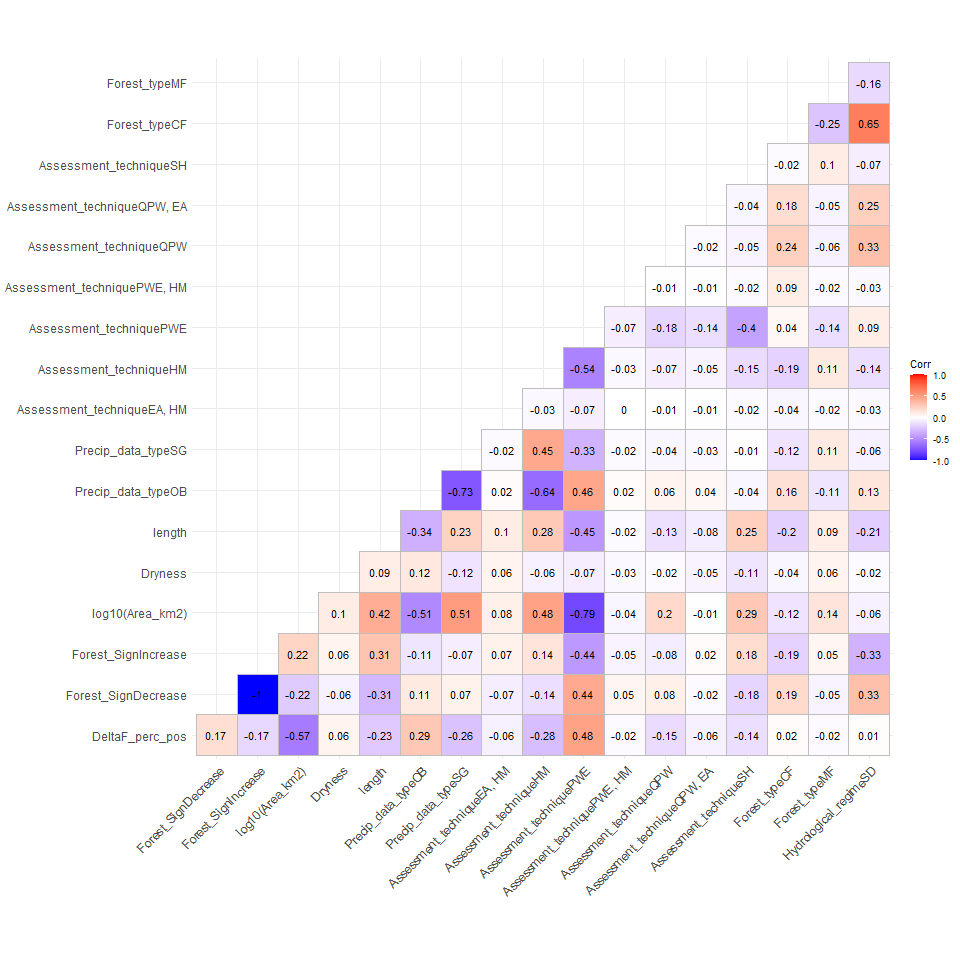
\includegraphics[width=0.9\linewidth]{./testcorr_plot} \caption{Correlation matrix for all variables}\label{fig:corgraphs}
\end{figure}

So the VIF really does not work, only works for numerical values and not for factor values. So this suggestion is not really relevant either.

However, being too focused on just the residual distribution can also lead to over fitting or over smoothing of the variables. This means that important characteristics of the data might be lost.

\textcolor{blue}{- The manuscript presents a number of alternative statistical models, differing by candidate explanatory variables. Each model is designed considering the key shortcomings of the previous one. The end result of such an approach is a complex and somewhat non systematic exploration of predictors and their explanatory power, where it is easy to get lost. I suggest restructuring the manuscript around a well-designed and robustly formalized model selection. One way to proceed could be to start with the most complex model suggested by the extant understanding of the processes at play, and then proceed with a model simplification, according to some consistent criteria (AIC, dropping non significant terms, or similar; high r2 is not a good criterion because it does not consider the number of parameters). A full blown model selection would also allow to retain or discard the interaction terms, which could be important (as also recognized by the authors; Section 4.5) and should not be discarded a priori. Doing a proper model selection and presenting the results only for the best model (according to a clearly specified criterion) would be less subjective and allow to drastically reduce the number of figures and tables, allowing the reader to focus their attention on the key message.}\\
\strut \\
As outlined in the last part of the reply, the focus of the statistical modelling in the paper is on understanding the different covariates that can explain the variation in the data.\\
\strut \\

\textcolor{blue}{- The novelty of this work needs to emerge more clearly in the introduction. As it looks now, the manuscript could be easily considered somewhat confirmatory, with respect to most data, approaches and conclusions reached by Zhang et al 2017 and Filoso et al 2017. Furthermore, the introduction needs to be rearranged, starting with a clear statement of the problem, what we know about that based on previous results, what is missing/how these previous analyses can be improved, and, stemming from these knowledge gaps and/or our understanding of the mechanisms, the questions addressed in the work or the hypotheses tested.}\\
\strut \\
This is a good point and we have rewritten the paper to strengthen this point.\\
\strut \\

\textcolor{blue}{There are also some typos and unfinished sentences (e.g., L 142, L 298). Some units are missing (for example those of length of the experiment in the figures) and symbols are not defined at their first appearance (E0/Pa in L 99; Dryness Index). Also: how is Table 1 used? These are not big issues per se but are nonetheless distracting.}

\textcolor{blue}{I would also like to provide the authors with a couple of suggestions regarding the statistical model and their interpretation. 
- The models used in the manuscript consider the absolute value of the forest cover change and then its sign, but this choice is not well justified. It implicitly assumes that the status corresponding to no change distinguishes two ‘realms’. Yet, I would expect (and it is also hinted at at some point in the manuscript) that what really matters is the \%forested area (possibly in relation to the climatic conditions) and how it changes. So, I would suggest the authors to consider whether a model nearer to our understanding of the phenomena at play would be one including, for the forest part, \%change in forested area (with sign) and \%forested area, with the latter possibly as random effect, if not of interested.}

\textcolor{blue}{- The fact that the explanatory power is low (low r2) does not necessarily make the results uninteresting (against conclusion on L 530), simply it suggests there are other factors, not included in the model, which have a large effect, and that the model presented cannot be used in a predictive mode. While it is important to present also the r2, even a model with low r2 square we learn which factors significantly affect the change in streamflow and which do not do so.}

\hypertarget{refs}{}
\begin{CSLReferences}{1}{0}
\leavevmode\vadjust pre{\hypertarget{ref-beck2013}{}}%
Beck, H. E., L. A. Bruijnzeel, A. I. J. M. van Dijk, T. R. McVicar, F. N. Scatena, and J. Schellekens. 2013. {``The Impact of Forest Regeneration on Streamflow in 12 Mesoscale Humid Tropical Catchments.''} Journal Article. \emph{Hydrol. Earth Syst. Sci.} 17 (7): 2613--35. \url{https://doi.org/10.5194/hess-17-2613-2013}.

\leavevmode\vadjust pre{\hypertarget{ref-birkinshaw2014}{}}%
Birkinshaw, Stephen J., James C. Bathurst, and Mark Robinson. 2014. {``45 Years of Non-Stationary Hydrology over a Forest Plantation Growth Cycle, Coalburn Catchment, Northern England.''} Journal Article. \emph{Journal of Hydrology} 519: 559--73. https://doi.org/\url{https://doi.org/10.1016/j.jhydrol.2014.07.050}.

\leavevmode\vadjust pre{\hypertarget{ref-brown2005}{}}%
Brown, Alice E., Lu Zhang, Thomas A. McMahon, Andrew W. Western, and Robert A. Vertessy. 2005. {``A Review of Paired Catchment Studies for Determining Changes in Water Yield Resulting from Alterations in Vegetation.''} Journal Article. \emph{Journal of Hydrology} 310 (1-4): 28--61. \url{http://www.sciencedirect.com/science/article/B6V6C-4G05MM9-1/2/bbc5fc0e958a8f34bcb7c1cc7fa57b48}.

\leavevmode\vadjust pre{\hypertarget{ref-cornish1993}{}}%
Cornish, P. M. 1993. {``The Effects of Logging and Forest Regeneration on Water Yields in a Moist Eucalypt Forest in New South Wales, Australia.''} Journal Article. \emph{Journal of Hydrology} 150 (2-4): 301--22. \href{http://www.sciencedirect.com/science/article/B6V6C-487D3Y2-9J/2/73c981ba76284d9d629f6b221d6fd6c6\%20}{http://www.sciencedirect.com/science/article/B6V6C-487D3Y2-9J/2/73c981ba76284d9d629f6b221d6fd6c6 }.

\leavevmode\vadjust pre{\hypertarget{ref-cornish2001}{}}%
Cornish, P. M., and R. A. Vertessy. 2001. {``Forest Age-Induced Changes in Evapotranspiration and Water Yield in a Eucalypt Forest.''} Journal Article. \emph{Journal of Hydrology} 242 (1-2): 43--63. \href{http://www.sciencedirect.com/science/article/B6V6C-429910G-3/2/0158b1f89ff436f338a9e688a47f06c4\%20}{http://www.sciencedirect.com/science/article/B6V6C-429910G-3/2/0158b1f89ff436f338a9e688a47f06c4 }.

\leavevmode\vadjust pre{\hypertarget{ref-filoso2017}{}}%
Filoso, Solange, Maíra Ometto Bezerra, Katherine C. B. Weiss, and Margaret A. Palmer. 2017. {``Impacts of Forest Restoration on Water Yield: A Systematic Review.''} Journal Article. \emph{PLOS ONE} 12 (8): e0183210. \url{https://doi.org/10.1371/journal.pone.0183210}.

\leavevmode\vadjust pre{\hypertarget{ref-hoekvandijke2022}{}}%
Hoek van Dijke, Anne J., Martin Herold, Kaniska Mallick, Imme Benedict, Miriam Machwitz, Martin Schlerf, Agnes Pranindita, Jolanda J. E. Theeuwen, Jean-François Bastin, and Adriaan J. Teuling. 2022. {``Shifts in Regional Water Availability Due to Global Tree Restoration.''} Journal Article. \emph{Nature Geoscience} 15 (5): 363--68. \url{https://doi.org/10.1038/s41561-022-00935-0}.

\leavevmode\vadjust pre{\hypertarget{ref-jackson2005}{}}%
Jackson, Robert B., Esteban G. Jobbagy, Roni Avissar, Somnath Baidya Roy, Damian J. Barrett, Charles W. Cook, Kathleen A. Farley, David C. le Maitre, Bruce A. McCarl, and Brian C. Murray. 2005. {``Trading Water for Carbon with Biological Carbon Sequestration.''} Journal Article. \emph{Science} 310 (5756): 1944--47. \url{https://doi.org/10.1126/science.1119282}.

\leavevmode\vadjust pre{\hypertarget{ref-jayasuriya1988}{}}%
Jayasuriya, M. D. A., and P. J. O'Shaughnessy. 1988. {``The Use of Mathematical Models in Evaluating Forest Treatment Effects on Streamflow.''} Book Section. In \emph{Hydrology and Water Resources Symposium 1988: Preprints of Papers,} 135--39. Hydrology; Water Resources Symposium. \url{https://doi.org/10.3316/informit.692214289455295}.

\leavevmode\vadjust pre{\hypertarget{ref-levy2018}{}}%
Levy, M. C., A. V. Lopes, A. Cohn, L. G. Larsen, and S. E. Thompson. 2018. {``Land Use Change Increases Streamflow Across the Arc of Deforestation in Brazil.''} Journal Article. \emph{Geophysical Research Letters} 45 (8): 3520--30. https://doi.org/\url{https://doi.org/10.1002/2017GL076526}.

\leavevmode\vadjust pre{\hypertarget{ref-oshaughnessy1979}{}}%
O'Shaughnessy, P. J., K. J. Langford, H. P. Duncan, and R. J. Moran. 1979. {``Catchment Experiments in Mountain Ash Forests at North Maroondah.''} Journal Article. \emph{Australian Forestry} 42 (3): 150--60. \url{https://doi.org/10.1080/00049158.1979.10674220}.

\leavevmode\vadjust pre{\hypertarget{ref-schneider1961}{}}%
Schneider, William Joseph, and Gordon Roundy Ayer. 1961. {``Effect of Reforestation on Streamflow in Central New York.''} Report 1602. \url{https://doi.org/10.3133/wsp1602}.

\leavevmode\vadjust pre{\hypertarget{ref-watson2001}{}}%
Watson, Fred, Rob Vertessy, Tom McMahon, Bruce Rhodes, and Ian Watson. 2001. {``Improved Methods to Assess Water Yield Changes from Paired-Catchment Studies: Application to the Maroondah Catchments.''} Journal Article. \emph{Forest Ecology and Management} 143 (1): 189--204. https://doi.org/\url{https://doi.org/10.1016/S0378-1127(00)00517-X}.

\leavevmode\vadjust pre{\hypertarget{ref-webb2009}{}}%
Webb, Ashley A. 2009. {``Streamflow Response to Pinus Plantation Harvesting: Canobolas State Forest, Southeastern Australia.''} Journal Article. \emph{Hydrological Processes} 23 (12): 1679--89. https://doi.org/\url{https://doi.org/10.1002/hyp.7301}.

\leavevmode\vadjust pre{\hypertarget{ref-webb2013}{}}%
Webb, Ashley A., and Brad W. Jarrett. 2013. {``Hydrological Response to Wildfire, Integrated Logging and Dry Mixed Species Eucalypt Forest Regeneration: The Yambulla Experiment.''} Journal Article. \emph{Forest Ecology and Management} 306: 107--17. https://doi.org/\url{https://doi.org/10.1016/j.foreco.2013.06.020}.

\leavevmode\vadjust pre{\hypertarget{ref-webb2012}{}}%
Webb, Ashley A., and Amrit Kathuria. 2012. {``Response of Streamflow to Afforestation and Thinning at Red Hill, Murray Darling Basin, Australia.''} Journal Article. \emph{Journal of Hydrology} 412-413: 133--40. https://doi.org/\url{https://doi.org/10.1016/j.jhydrol.2011.05.033}.

\leavevmode\vadjust pre{\hypertarget{ref-zhang2017}{}}%
Zhang, Mingfang, Ning Liu, Richard Harper, Qiang Li, Kuan Liu, Xiaohua Wei, Dingyuan Ning, Yiping Hou, and Shirong Liu. 2017. {``A Global Review on Hydrological Responses to Forest Change Across Multiple Spatial Scales: Importance of Scale, Climate, Forest Type and Hydrological Regime.''} Journal Article. \emph{Journal of Hydrology} 546: 44--59. https://doi.org/\url{https://doi.org/10.1016/j.jhydrol.2016.12.040}.

\leavevmode\vadjust pre{\hypertarget{ref-zhou2015}{}}%
Zhou, Guoyi, Xiaohua Wei, Xiuzhi Chen, Ping Zhou, Xiaodong Liu, Yin Xiao, Ge Sun, et al. 2015. {``Global Pattern for the Effect of Climate and Land Cover on Water Yield.''} Journal Article. \emph{Nature Communications} 6 (1): 5918. \url{https://doi.org/10.1038/ncomms6918}.

\end{CSLReferences}


\end{document}
